\documentclass[12pt,a4paper]{article}
\usepackage[UTF8]{ctex}
\usepackage{amsmath,amssymb}
\usepackage{listings}
\usepackage{xcolor}
\usepackage{hyperref}
\usepackage{geometry}
\usepackage{graphicx}
\geometry{margin=2.5cm}

\lstdefinestyle{python}{
  language=Python,
  basicstyle=\ttfamily\small,
  keywordstyle=\color{blue}\bfseries,
  commentstyle=\color{gray},
  stringstyle=\color{red},
  showstringspaces=false,
  breaklines=true,
  frame=single,
  backgroundcolor=\color{gray!10}
}

\title{Quantum Annealing / 量子退火}
\author{QuoNic}
\date{}

\begin{document}
\maketitle

\begin{center}
\textbf{Algorithms / 算法} | 难度：中级 | 预计时间：15 分钟
\end{center}

\tableofcontents
\newpage

\section{为什么需要？}

量子退火是解决组合优化问题的量子算法，是 D-Wave 量子计算机的核心。

\subsection{经典局限}
\b\begin{itemize}
  \item 经典模拟退火容易陷入局部最优
  \item 对于复杂能量景观，经典方法效率低
\end{itemize}

\subsection{量子优势}
\b\begin{itemize}
  \item 量子退火利用量子隧穿效应逃离局部最优
  \item 对于某些问题，量子退火比经典方法更快
  \item 是 D-Wave 量子计算机的核心算法
\end{itemize}

\subsection{实际应用}
\b\begin{itemize}
  \item 组合优化（MaxCut、TSP）
  \item 机器学习（训练玻尔兹曼机）
  \item 金融（投资组合优化）
\end{itemize}

\section{快速上手}

\begin{lstlisting}[style=python]
from quonic.algorithms import quantum_annealing

# Define optimization problem
problem = {"0-1": -1, "1-2": -1, "2-3": -1}

# Run quantum annealing
result = quantum_annealing(problem, steps=100)
print(f"Solution: {result.solution}")
print(f"Energy: {result.energy}")
\end{lstlisting}

\textbf{预期输出}：
\begin{verbatim}
Solution: [1, 0, 1, 0]
Energy: -3
\end{verbatim}

\section{原理详解}

\subsection{电路图}

\begin{center}
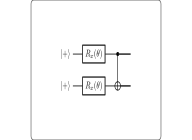
\includegraphics[width=0.6\textwidth]{../../images/quantum_annealing_circuit.svg}
\end{center}

\subsection{数学推导}

量子退火的哈密顿量：
\begin{equation}
H(t) = (1 - t/T) H_0 + (t/T) H_P
\end{equation}

其中 $H_0$ 是初始哈密顿量（横向场），$H_P$ 是问题哈密顿量。

\textbf{退火过程}：
\begin{enumerate}
  \item 从 $H_0$ 的基态开始
  \item 缓慢演化到 $H_P$
  \item 绝热定理保证系统保持在基态
  \item 最终测量得到 $H_P$ 的基态
\end{enumerate}

\subsection{几何解释}

量子退火在能量景观中寻找最低点。量子隧穿效应允许系统穿过能量壁垒，逃离局部最优。

\section{代码详解}

\begin{lstlisting}[style=python]
from quonic.algorithms import quantum_annealing

# quantum_annealing(problem, steps, shots)
# problem: dictionary of couplings {(i,j): weight}
# steps: number of annealing steps
# shots: number of measurements
result = quantum_annealing(problem, steps=100, shots=1024)

# result.solution: bit string solution
# result.energy: energy of solution
# result.history: annealing history
print(f"Solution: {result.solution}")
\end{lstlisting}

\section{进阶用法}

\subsection{场景 1：不同问题}

\begin{lstlisting}[style=python]
# MaxCut problem
problem = {"0-1": -1, "1-2": -1, "2-0": -1}
result = quantum_annealing(problem, steps=100)

# TSP problem
from quonic.optimization import tsp_to_qubo
problem = tsp_to_qubo(cities)
result = quantum_annealing(problem, steps=200)
\end{lstlisting}

\subsection{场景 2：不同步数}

\begin{lstlisting}[style=python]
# More steps for better results
result_100 = quantum_annealing(problem, steps=100)
result_500 = quantum_annealing(problem, steps=500)
result_1000 = quantum_annealing(problem, steps=1000)
\end{lstlisting}

\section{适用场景}

\subsection{组合优化}

量子退火可以用于各种组合优化问题。

\subsection{机器学习}

量子退火可以用于训练玻尔兹曼机。

\subsection{金融}

量子退火可以用于投资组合优化。

\section{常见问题}

\subsection{量子退火和 QAOA 有什么区别？}

量子退火是连续时间演化，QAOA 是离散时间演化。量子退火用 D-Wave 硬件，QAOA 用门模型硬件。

\subsection{量子退火能保证最优解吗？}

理论上，绝热定理保证系统保持在基态。但实际中，退火速度有限，可能跳出基态。

\section{学习路径}

\subsection{前置知识}
\b\begin{itemize}
  \item 组合优化基础
  \item 哈密顿量
  \item 绝热定理
\end{itemize}

\subsection{继续学习}
\b\begin{itemize}
  \item QAOA
  \item 量子优化
  \item D-Wave 编程
\end{itemize}

\section{完整示例代码}

\subsection{示例 1：基本量子退火}

\begin{lstlisting}[style=python]
from quonic.algorithms import quantum_annealing

problem = {"0-1": -1, "1-2": -1, "2-3": -1}
result = quantum_annealing(problem, steps=100)
print(f"Solution: {result.solution}")
\end{lstlisting}


\section{下载}

\begin{itemize}
  \item [quantum_annealing.py](https://github.com/ChrisLee0721/QuoNic/blob/main/examples/quantum_annealing/quantum_annealing.py)
\end{itemize}

\end{document}
